% !TeX root = interim.tex
% ***************************** さわるな(ここから)************

% 基本設定 ==============================================
\documentclass[9pt,dvipdfmx,uplatex]{jsarticle}
\usepackage{graphicx}
\usepackage[top=15truemm,bottom=20truemm,left=15truemm,right=15truemm]{geometry}
\pagestyle{empty}
\usepackage{enumerate}
\usepackage{txfonts}
\usepackage{xurl}
\usepackage[deluxe]{otf}
\doublerulesep=\arrayrulewidth
\setlength\intextsep{0pt}
\setlength\floatsep{0pt} %dblfloatsep
\setlength\textfloatsep{0pt} %dbltextfloatsep
\renewcommand{\baselinestretch}{0.8} % 行間

% 見出し上下の余白などの調整 ===========================
\makeatletter
\def\section{\@startsection {section}{1}{\z@}
{0.6zh}%余白上
{0.5zh}%余白下
 {\normalsize\bfseries\gtfamily}%体裁
 }
\def\subsection{\@startsection {subsection}{1}{\z@}
{1ex plus -1ex minus-.2ex}%余白上
{0ex plus 1.2ex}%余白下
 {\normalsize\bfseries\gtfamily}%体裁
 }
\makeatother
% section/subsectionの調整
\renewcommand{\thesection}{\arabic{section}.\hskip-4pt}
\renewcommand{\thesubsection}{\arabic{section}.\arabic{subsection}.\hskip0pt}

% 参考文献 ===========================
\renewcommand{\refname}{参考文献} 

% ***************************** さわるな(ここまで)************

\begin{document}
% タイトル =====================================
\twocolumn[
\vspace{-5mm}
\begin{flushright}
(鷹合研)
\end{flushright}
\begin{center}
{\Large\bfseries\gtfamily 学生のやるやる詐欺を黙認する方法}\vspace{2mm}
\end{center}
% 著者情報 =====================================
\begin{minipage}{185mm}
\begin{center}
3EP5-01 武田 晴信,3EP5-19 武田 信繁,3EP5-99 武田 信廉
\end{center}
\end{minipage}
\vspace{3mm}
] 
% 本文  =========================================
\section{はじめに}
レポートは見栄え良く書くことが求められます.レポートは見栄え良く書くことが求められます.レポートは見栄え良く書くことが求められます.

レポートは用紙全体をうめるように書きましょう.スカスカだと中味がないと思われてしまいます.

空行を入れると新しい段落ができます.空行を入れると新しい段落ができます.空行を入れると新しい段落ができます.空行を入れると新しい段落ができます.空行を入れると新しい段落ができます.空行を入れると新しい段落ができます.

参考文献はこうする\cite{REF_XXX}.参考文献はこうする\cite{REF_ABC,bk1}.よくわからなければインターネットで書き方を調べてみましょう.

% section 2 ----
\section{予測式形状と参照領域サイズを選択する方法}
\subsection{箇条書きの書き方}
番号付き箇条書きの例です.番号付き箇条書きの例です.番号付き箇条書きの例です.
\begin{enumerate}
	\item りんご
	\item みかん
	\item なし
\end{enumerate}


番号なし箇条書きの例です.番号なし箇条書きの例です.番号なし箇条書きの例です.
\begin{itemize}
	\item りんご
	\item みかん
	\item なし
\end{itemize}

特定の項目に対して説明をする場合.特定の項目に対して説明をする場合.特定の項目に対して説明をする場合.
\begin{description}
	\item[りんご] ああああああああああああああああああああああああああああああああああああああああああ
	\item[みかん] いいいいいいいいいいいいいいいいいいいいいいいいいいいいいいいいいいいいいいいいいい
	\item[なし] ううううううううううううううううううううううううううううううううううううううう
\end{description}
\subsection{図の参照方法}
りんごとみかんを図\ref{FIG_YYY},図\ref{FIG_ZZZ}にそれぞれ示す.ラベルを使って丁寧に書きましょう.

\subsection{表の参照方法}
表\ref{TBL_AAA}はゼミの遅刻者リストである.ラベルを使って丁寧に書きましょう.ラベルを使って丁寧に書きましょう.



\subsection{式の書き方}
$N$を入力信号$x_b(n)$の長さとする.
式は少々面倒ですが美しく書けます.

\begin{equation}\label{EQ_ABC}
S_b(p,L)=\sum_{n=0}^{N-1} \left\{ x_b(n)-\hat{x_b}_{p,L}(n) \right\}^2
\end{equation}

ここで,式(\ref{EQ_ABC})の右辺を整理すると
\begin{equation}
S_b(p,L)=1.0
\end{equation}
が得られる.


\section{実験結果}
ああああああああああああああああああああああああああああああああああああ.いいいいいいいいいいい.ううううううううう.

ええええええええええええ.おおおおおおおおおおおおおおおおおおおお.

かかかかかかかかかかかかかかかかかかかかかかかかかかかかかかかかかかかかかかかかかかかかかかかかかかかかかかかかかかかかかかかかかかかかかかかかかかかかかかかかかかかかかかかかかかかかかかかかかかかかかかかかかかかかかかかかかかかかかかかかかかかかかかかかかかかかかかかかかかかかかかかかかかかかかかかかかかかかかかかかかかかかかかかかかかかかかかかかかかかかかかかかかかかかかかかかかかかかか.



\section{まとめ}
ああああああああああああああああああああああああああああああああああああ.いいいいいいいいいいい.ううううううううう.

ええええええええええええ.おおおおおおおおおおおおおおおおおおおお.


% ==============================================
% 原稿はここまで
% ==============================================
\begin{figure}[t]
   \begin{center}
    \vspace{5mm}
   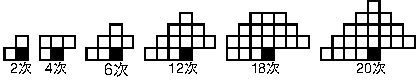
\includegraphics[width=0.4\textwidth]{fig/fig1.pdf}
   \caption{予測式の形状$p$, 左から$p=0,1,2,3,4,5$とする}
   \label{FIG_YYY}
%
   \vspace{2mm}
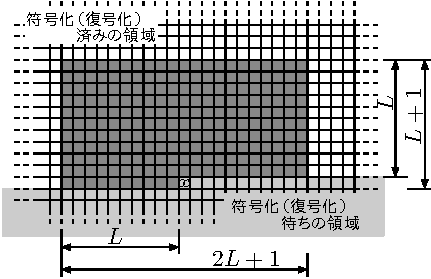
\includegraphics[width=0.43\textwidth]{fig/fig2.pdf}
\caption{注目画素$x$の予測式係数決定に使われる領域, $L=10,11,\cdots19$とする}
\label{FIG_ZZZ}
   \end{center}
\end{figure}

\begin{table}[t]
\begin{center}
\caption{5種の画像に対する予測誤差のエントロピ}\label{TBL_AAA}
\begin{tabular}{lcccc}
\noalign{\hrule height 1pt}
標準画像 & あ & い & え &お\\
\noalign{\hrule height 1pt} 
barbara &4.314&4.331&4.406&4.496\\
        &(4.291)&(4.325)&\\\hline
lenna   &3.913&3.915&3.951&3.956\\
        &(3.890)&(3.909)\\\hline
airplane&4.021&4.027&4.075&4.058\\
        &(3.998)&(4.021)\\\hline
peppers &4.426&4.442&4.491&4.491\\
        &(4.403)&(4.436)\\\hline
girl    &4.368&4.373&4.408&4.442\\
        &(4.345)&(4.367)\\
\noalign{\hrule height 1pt}
\end{tabular}\\
括弧内はオーバーヘッドを含めないときのエントロピ
\end{center}
\end{table}


\begin{thebibliography}{99}
\bibitem{REF_XXX}小松 邦紀, 瀬崎 薫, 安田 靖彦, ``濃淡画像の可逆的なサブ
バンド符号化法'', 信学論(D-II), vol.J78-D-II, no.3,
pp.429-436, March 1995.
\bibitem{REF_ABC}A.R. Calderbank, I. Daubechies, W. Sweldens and B. Yeo, ''Lossless
image compression using integer to integer wavelet transforms,'' 
IEEE Proc. ICIP 97, vol.1, pp.596-599, 1997.
\bibitem{bk1} "金沢の暮らし", \url{http://www.kanazawa-it.ac.jp}
\end{thebibliography}

\end{document}
